\documentclass{beamer}
\usepackage{ucs}
\usepackage[utf8x]{inputenc}
\usepackage[T1]{fontenc}
\usepackage[spanish]{babel}
\usepackage{listings}
\usetheme{Darmstadt}
\usecolortheme{whale}
\setbeamercovered{transparent}

\usepackage{color}
\definecolor{gray97}{gray}{.97}
\definecolor{gray75}{gray}{.75}
\definecolor{gray45}{gray}{.45}
 
\usepackage{listings}
\lstset{ frame=Ltb,
     framerule=0pt,
     aboveskip=0.5cm,
     framextopmargin=3pt,
     framexbottommargin=3pt,
     framexleftmargin=0.4cm,
     framesep=0pt,
     rulesep=.4pt,
     backgroundcolor=\color{gray97},
     rulesepcolor=\color{black},
     %
     stringstyle=\ttfamily,
     showstringspaces = false,
     basicstyle=\small\ttfamily,
     commentstyle=\color{gray45},
     keywordstyle=\bfseries,
     %
     numbers=left,
     numbersep=15pt,
     numberstyle=\tiny,
     numberfirstline = false,
     breaklines=true,
   }
 
% minimizar fragmentado de listados
\lstnewenvironment{listing}[1][]
   {\lstset{#1}\pagebreak[0]}{\pagebreak[0]}
 
\lstdefinestyle{consola}
   {basicstyle=\scriptsize\bf\ttfamily,
    backgroundcolor=\color{gray75},
   }
 
%\lstdefinestyle{C}
%   {language=C,
%   }

\title{"Sistema Automatizado de Ventas bajo el framework Ruby on Rails" \\ Capítulo 1 y 2}
\author{
    Bernardo Arancibia Araos
        \and Sebastián Machuca Sáez
}
\institute{
    Técnico Universitario en Informática \\ \vspace*{0.3cm}
    
\includegraphics[width=0.2\textwidth]{images/utfsm.png} \\ \vspace*{0.3cm} \tiny{Sede José Miguel Carrera} \\ 
        VIÑA DEL MAR 
}
\date{5 de Julio de 2010}

%%%%%%% DOCUMENTO %%%%%%%%%%%%%%%%%%%%

\begin{document}

\begin{frame}
\maketitle
\end{frame}

\begin{frame}
\frametitle{Introducción}
\begin{itemize}

\item Pymes sin acceso a tecnología <> Grandes Empresas 
\item Expansión de Internet 
\item Cualidades del concepto \emph{Web 2.0} 
\end{itemize}
\end{frame}

\section{Aspectos relevantes del diseño lógico}

\begin{frame}
\textbf{Capítulo 1}

\mbox{}

Aspectos relevantes del diseño lógico
\end{frame}

\subsection{Descripción de la organización}

\begin{frame}
\frametitle{Descripción de la organización}
\begin{itemize}
\item \textbf{Nombre:} Provisiones Frutas y Verduras \emph{Chusmisa}
\item \textbf{Ubicación:} Población El Olivar, Viña del Mar
\item \textbf{Rubro:} Venta de Abarrotes
\end{itemize}
\end{frame}

\begin{frame}
\frametitle{Entes componentes del funcionamiento de la organización}
\begin{itemize}
\item Administrador
\item Vendedor
\item Proveedores
\end{itemize}
\end{frame}

\begin{frame}
\frametitle{Herramientas de trabajo actual}
\begin{itemize}
\item Balanzas Digitales
\item Refrigeradores
\item Cuadernos y hojas
\item \alert{Una Computadora}
\item \alert{Internet}
\end{itemize}
\end{frame}

\subsection{Descripción de la situación actual}

\begin{frame}
\frametitle{Descripción de la situación actual}
Se pueden identificar los siguientes procesos:
\begin{enumerate}
\item Proceso de ventas                       
\item Proceso de devolución de productos 
\item Proceso de compra de productos mediante crédito informal 
\item Proceso de registro de pedidos 
\item Proceso de cálculo de libro de ventas 
\item Proceso de compra a proveedores 
\item Proceso de control de stock
\end{enumerate}
\end{frame}

\subsection{Problemas detectados}

\begin{frame}
\frametitle{Problemas detectados}
\begin{itemize}
\item Centralización de precios e información del negocio en una sola persona. 
\item No existe control de salida e ingreso de productos (stock). 
\item Ventas con crédito informal y pedidos se administran de forma desordenada. 
\item Falta de automatización en ciertas tareas.
\end{itemize}
\end{frame}

%%%%%%%%%%%%%%%%%%%%% ARREGLAR

\subsection{Objetivos del sistema propuesto}

\begin{frame}
\begin{itemize}
\frametitle{Objetivo principal del sistema propuesto}
\item Sistema integrado que automatice:
\begin{itemize}
\item Gestión de ventas
\item Administración de productos y perfiles de usuario
\end{itemize}
\item \emph{Vitrina Online}
\end{itemize}
\end{frame}

\begin{frame}
\begin{itemize}
\frametitle{Objetivo específico del sistema propuesto}
\item Generar y accesar una \emph{Base de Datos} 
\item Generar informe de ventas 
\item Control en el flujo de dinero y productos
\item Listar y procesar ventas con crédito informal
\item Listar y procesar pedidos
\item \alert{Crear una interfaz gráfica que implique un ágil proceso
para los \textbf{vendedores} y una interfaz de \emph{Vitrina Online} de 
fácil uso para los \textbf{clientes}}
\end{itemize}
\end{frame}

\subsection{Estructura funcional del sistema propuesto}

\begin{frame}
\frametitle{Estructura funcional del sistema propuesto}
Mantenedores: 
\begin{enumerate}
\item Vendedores
\item Notas
\item Proveedores
\item Clientes 
\item Productos 
\item Pedidos 
\item Ventas
\item Venta a crédito informal 
\item Mermas
\item Categorías
\end{enumerate}
\end{frame}

\begin{frame}
Otras funcionalidades: 
\begin{enumerate}
\item Generar Libro de Ventas.
\item Control de devoluciones. 
\item Realizar arqueo de caja
\end{enumerate}
\end{frame}

\subsection{Entradas}

\begin{frame}
\frametitle{Entradas}
\begin{enumerate}
\item Datos de proveedor
\item Datos de vendedor
\item Datos de una nota
\item Datos de cliente
\item Datos de producto
\item Datos de categoría
\item Datos de crédito
\item Datos de pedido
\item Datos de venta
\item Datos de merma
\end{enumerate}
\end{frame}

\subsection{Salidas}

\begin{frame}
\frametitle{Salidas}
\begin{enumerate}
\item Listado de proveedores
\item Listado de vendedores
\item Listado de notas por vendedor
\item Listado de notas de todos los vendedores
\item Listado de notas por fecha y hora 
\item Listado de clientes 
\item Listado de clientes con crédito 
\item Listado de clientes por pedido 
\item Listado de productos 
\item Listado de productos por tipo 
\item Listado de productos por stock (crítico) 
\item Listado de productos por categoría
\end{enumerate}
\end{frame}

\subsection{Entidades de Información}

\begin{frame}
\frametitle{Entidades de Información}
\begin{enumerate}
\item Vendedores
\item Clientes
\item Proveedores
\item Productos
\item Categorías
\item Ventas 
\item Detalles Ventas
\item Pedidos
\item Detalles Pedidos 
\item Créditos
\item Mermas  
\item Notas
\end{enumerate}
\end{frame}

\begin{frame}
\begin{center}
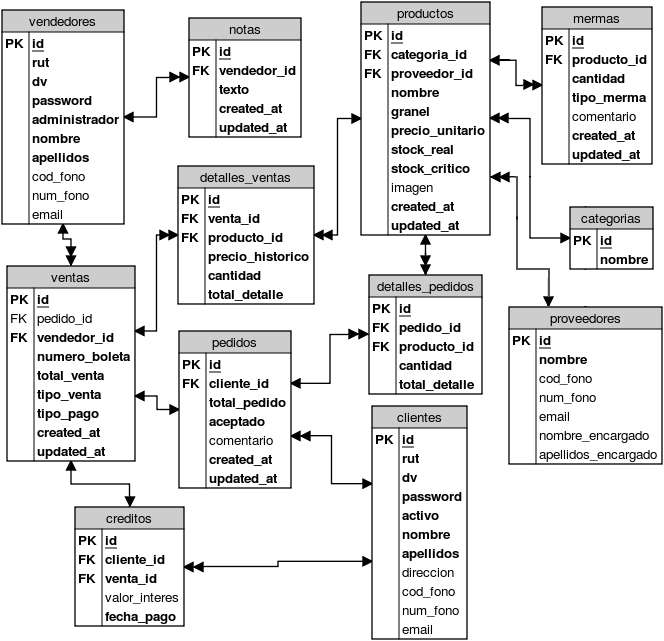
\includegraphics[width=0.8\textwidth]{images/modelo_relacional.png}
\end{center}
\end{frame}

\section{Medio ambiente computacional y descripción de archivos}

\begin{frame}
\textbf{Capítulo 2}

\mbox{}

Medio ambiente computacional y descripción de archivos
\end{frame}

\subsection{Características del recurso computacional}

\begin{frame}
\frametitle{Configuración del sistema}

\begin{enumerate}
\item \textbf{Hosting básico Heroku}
\begin{itemize}
\pause
\item 5MB Espacio Base de Datos 
\item 100 MB Espacio archivos\pause
\end{itemize}

\item \textbf{Equipo Cliente Local}
\begin{itemize}
\item Procesador Athlon XP 1.8 Ghz
\item Disco Duro 20 GB
\item Memoria RAM 256 MB \pause
\end{itemize}

\item \textbf{Equipo desarrollo 1}
\begin{itemize}
\item Acer Aspire 4535
\item Procesador Turion X2 2.1 Ghz
\item Disco Duro 320 GB
\item Memoria RAM 3 GB \pause
\end{itemize}

\item \textbf{Equipo desarrollo 2}
\begin{itemize}
\item Dell Inspiron 1420
\item Procesador Core 2 Duo 1.6 Ghz
\item Disco Duro 120 GB
\item Memoria RAM 2 GB
\end{itemize}

\end{enumerate}

\end{frame}

\begin{frame}
\textbf{Requisitos Mínimos}
\begin{itemize}
\item Procesador a 500 Mhz
\item Disco Duro 100 MB
\item Memoria RAM 256
\item Conexión a Internet de 512 Kbps 
\item Navegador Web compatible con Javascript
\end{itemize}
\end{frame}

\subsection{Software Utilizado}

\begin{frame}
\frametitle{Sistema Operativo}
\begin{itemize}
\item GNU/Linux
\begin{enumerate}
\pause
\item \textbf{Equipo Cliente:} Debian GNU/Linux \pause
\item \textbf{Equipo de desarrollo 1:} Open Suse GNU/Linux, v. 11.2 \pause
\item \textbf{Equipo de desarrollo 2:} Archlinux GNU/Linux, v. 2010 \pause
\end{enumerate}
\end{itemize}
\end{frame}

\begin{frame}
\frametitle{Herramientas de desarrollo de Software}
\begin{enumerate}
\pause
\item \alert{Ruby on Rails} \pause
\item \alert{PostgreSQL (Con ORM ActiveRecord)} \pause
\item JQuery \pause
\item GIT \pause
\item Gema Heroku \pause
\item VIM
\end{enumerate}
\end{frame}

\begin{frame}
\frametitle{ActiveRecord - Convenciones}
Ejemplo de Convenciones
\begin{itemize}
\item \textbf{Vendedor} : La Clase
\item \textbf{vendedores} : La Tabla
\item \textbf{id} : nombre de clave primaria 
\item \textbf{vendedor\_id} : nombre clave foránea
\end{itemize}
\end{frame}

\begin{frame}
Archivo db/schema.rb
\lstinputlisting[language=Ruby]{code/schema.rb}
\end{frame}

\begin{frame}
Archivo app/model/vendedor.rb
\lstinputlisting[language=Ruby]{code/vendedor.rb}
\end{frame}

\begin{frame}
Archivo app/model/notas.rb
\lstinputlisting[language=Ruby]{code/notas.rb}
\end{frame}

\begin{frame}
\frametitle{Lenguaje de Comandos}
\begin{enumerate}
\item Bash \pause
\item Rails Console
\end{enumerate}
\end{frame}

\subsection{Descripción detallada de tablas}

\begin{frame}
\frametitle{Descripción detallada de tablas}
\begin{enumerate}
\item \alert{Ventas}
\item \alert{Detalles Ventas}
\item \alert{Vendedores}
\item \alert{Productos} \pause
\item Clientes
\item Proveedores
\item Pedidos
\item Detalles Pedidos
\item Categorías
\item Créditos
\item Mermas
\item Notas
\end{enumerate}
\end{frame}

\begin{frame}
\frametitle{Tabla Ventas}
\begin{figure}
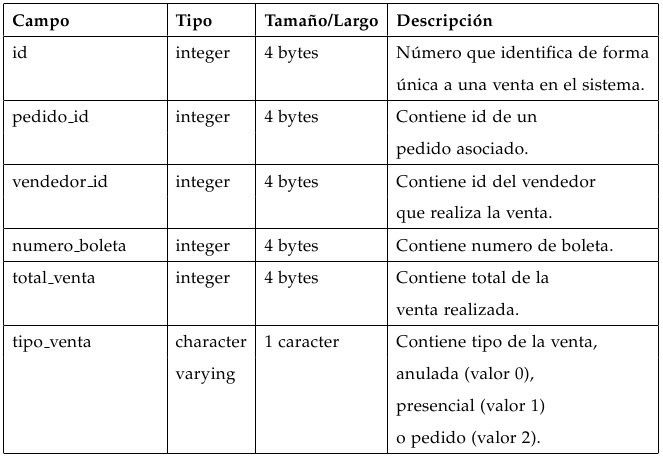
\includegraphics[width=0.7\textwidth]{images/tabla_ventas1.jpg}
\caption{Campos Tabla Ventas \tiny{(img. 1 de 2)}}
\end{figure}
\end{frame}

\begin{frame}
\frametitle{Tabla Ventas}
\begin{figure}
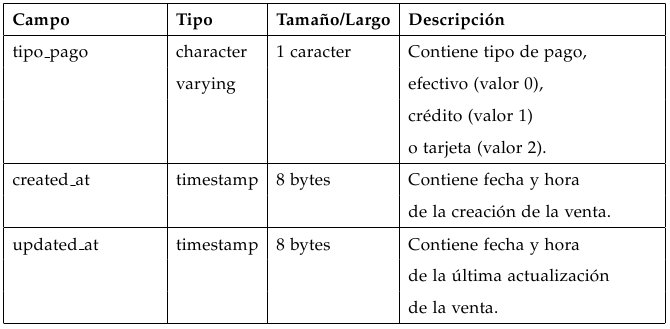
\includegraphics[width=0.7\textwidth]{images/tabla_ventas2.jpg}
\caption{Campos Tabla Ventas \tiny{(img. 1 de 2)}}
\end{figure}
\end{frame}

\begin{frame}
\frametitle{Tabla Detalles Ventas}
\begin{figure}
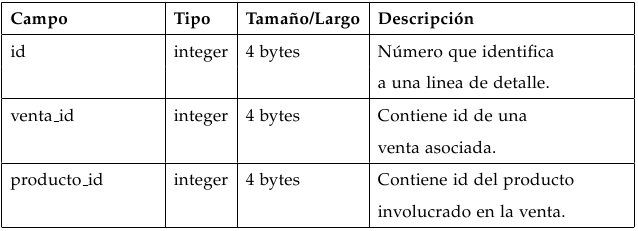
\includegraphics[width=0.7\textwidth]{images/tabla_detalles_ventas1.jpg}
\caption{Campos Tabla Detalles Ventas \tiny{(img. 1 de 2)}}
\end{figure}
\end{frame}

\begin{frame}
\frametitle{Tabla Detalles Ventas}
\begin{figure}
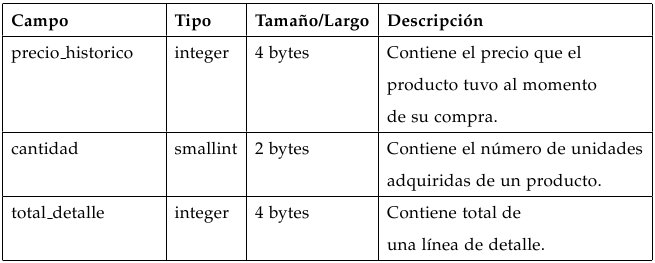
\includegraphics[width=0.7\textwidth]{images/tabla_detalles_ventas2.jpg}
\caption{Campos Tabla Detalles Ventas \tiny{(img. 2 de 2)}}
\end{figure}
\end{frame}


\begin{frame}
\frametitle{Tabla Vendedores}
\begin{figure}
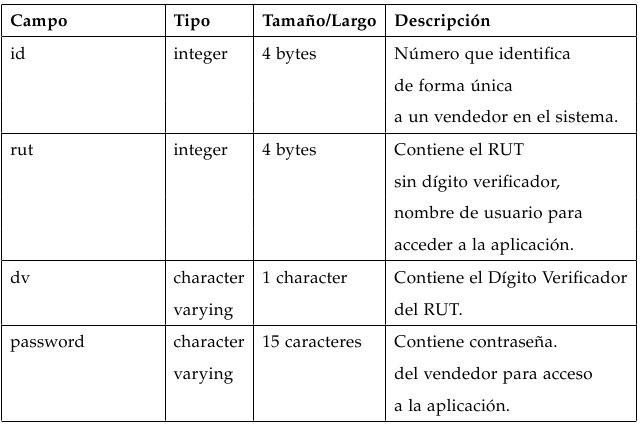
\includegraphics[width=0.7\textwidth]{images/tabla_vendedores1.jpg}
\caption{Campos Tabla Vendedores \tiny{(img. 1 de 2)}}
\end{figure}
\end{frame}

\begin{frame}
\frametitle{Tabla Vendedores}
\begin{figure}
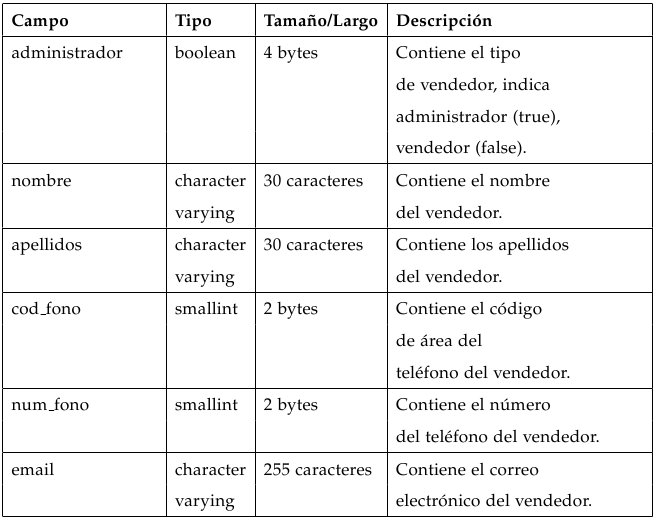
\includegraphics[width=0.7\textwidth]{images/tabla_vendedores2.jpg}
\caption{Campos Tabla Vendedores \tiny{(img. 2 de 2)}}
\end{figure}
\end{frame}


\begin{frame}
\frametitle{Tabla Productos}
\begin{figure}
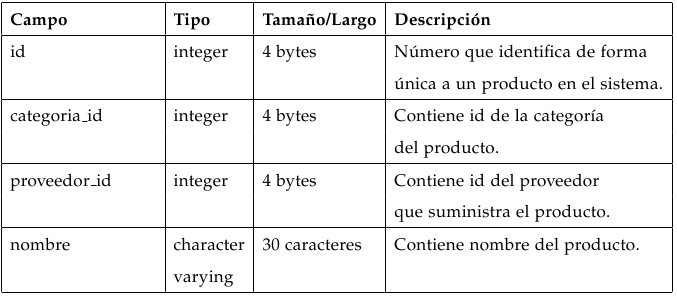
\includegraphics[width=0.7\textwidth]{images/tabla_productos1.jpg}
\caption{Campos Tabla Productos \tiny{(img. 1 de 2)}}
\end{figure}
\end{frame}

\begin{frame}
\frametitle{Tabla Productos}
\begin{figure}
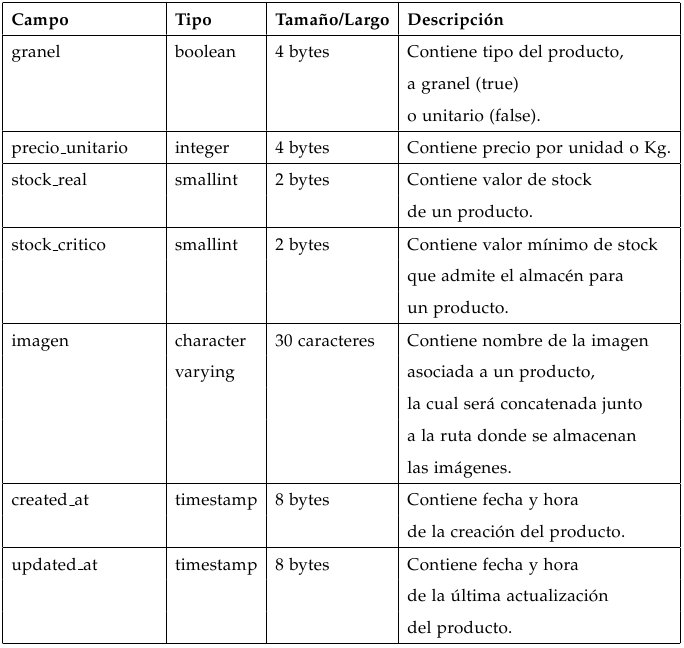
\includegraphics[width=0.7\textwidth]{images/tabla_productos2.jpg}
\caption{Campos Tabla Productos \tiny{(img. 2 de 2)}}
\end{figure}
\end{frame}

\subsection{}
\begin{frame}
\begin{center}
\huge{\textbf{FIN}}
\end{center}
\end{frame}

\end{document}
